\documentclass{beamer}

\usepackage[utf8]{inputenc}
%\usepackage{beamerthemesplit}
\usepackage{url}
\usepackage{tikz}
\usepackage{alltt}
\usepackage{listings}
\usepackage{marvosym}
\usepackage{color}
\usepackage[multidot]{grffile}
\usepackage{multirow}
\usepackage{array}
\usepackage{setspace}
\usepackage{hyperref}
\usepackage{verbatim}
\usepackage{fancyvrb}
%\hypersetup{colorlinks=true, linkcolor=blue,  anchorcolor=blue,  
%citecolor=blue, filecolor=blue, menucolor=blue, pagecolor=blue,  
%urlcolor=blue} 
\lstset{keywordstyle=\bfseries\color{brown},
        stringstyle=\ttfamily,
        commentstyle=\color{blue}\textit,
        showstringspaces=false}

\useoutertheme{}
\usetheme{Madrid}
\graphicspath{{pics/}{global/}
{pics/I/}{pics/A1/}{pics/A2/}{pics/A3/}{pics/A4/}{pics/A5/}{pics/A6/}{pics/A7/}
}

\logo{
\includegraphics[height=1cm]{ProcessHorizontal}} 

\institute{Center for Computation and Technology\\Louisiana State University, Baton Rouge, LA}

\setbeamertemplate{navigation symbols}{} 

\title{CSC 7700: Scientific Computing}

% We want to use the infolines outer theme because it does not use a lot of
% space, but it also tries to print an institution and the slide
% numbers (which we might not want to show). Therefore, we here redefine the
% footline ourselfes - mostly a copy & paste from
% /usr/share/texmf/tex/latex/beamer/themes/outer/beamerouterthemeinfolines.sty
\defbeamertemplate*{footline}{infolines theme without institution and slide numbers}
{
  \leavevmode%
  \hbox{%
  \begin{beamercolorbox}[wd=.25\paperwidth,ht=2.25ex,dp=1ex,center]{author in head/foot}%
    \usebeamerfont{author in head/foot}\insertshortauthor
  \end{beamercolorbox}%
  \begin{beamercolorbox}[wd=.5\paperwidth,ht=2.25ex,dp=1ex,center]{title in head/foot}%
    \usebeamerfont{title in head/foot}\insertshorttitle
  \end{beamercolorbox}%
  \begin{beamercolorbox}[wd=.25\paperwidth,ht=2.25ex,dp=1ex,center]{date in head/foot}%
    \usebeamerfont{date in head/foot}\insertshortdate{}
  \end{beamercolorbox}}%
  \vskip0pt%
}

% Some useful commands
\newcommand{\abspic}[4]
 {\vspace{ #2\paperheight}\hspace{ #3\paperwidth}\includegraphics[height=#4\paperheight]{#1}\\
  \vspace{-#2\paperheight}\vspace{-#4\paperheight}\vspace{-0.0038\paperheight}}

\newcommand{\picw}[4]{{
 \usebackgroundtemplate{
 \color{black}\vrule width\paperwidth height\paperheight\hspace{-\paperwidth}\hspace{-0.01\paperwidth}
 \hspace{#4\paperwidth}\includegraphics[width=#3\paperwidth, height=\paperheight]{#1}}\logo{}
 \frame[plain]{\frametitle{#2}}
}}
\newcommand{\pic}[2]{\picw{#1}{#2}{}{0}}

\newcommand{\question}[1]{\frame{\frametitle{#1}
 \begin{centering}\Huge #1\\\end{centering}
}}



\subtitle[Module A]{{\large Module A: Basic Skills}\\*[0.3em]Lecture 2: Collaboration management, Programming best practices}
\author[\mbox{
\includegraphics[height=0.6em]{fl_300}\hspace{0.5em}Frank Löffler}]{Dr Frank Löffler}
\date{Sep 06 2013}
\usecolortheme[RGB={234,110,0}]{structure}

\begin{document}

\setbeamercolor{alerted text}{fg=gray,bg=}

\frame{\titlepage}

\section{Overview}
\frame{\frametitle{}\begin{centering}\LARGE\insertsectionhead\\\end{centering}}

\frame[containsverbatim]{ \frametitle{Overview}
 Software development, or
 \begin{itemize}
  \item Application Development
  \item Software Design
  \item Software Engineering
  \item Software Application Development
  \item Enterprise Application Development
  \item Platform Development
 \end{itemize}
 ... development of a software product in a planned and structured process.
}

\frame[containsverbatim]{ \frametitle{Overview}
 Software development involves some combination of stages:
 \begin{itemize}
  \item Market research
  \item Gathering requirements for the proposed business solution
  \item Analyzing the problem
  \item Devising a plan or design for the software-based solution
  \item Implementation (coding) of the software
  \item Testing the software
  \item Deployment
  \item Maintenance and bug fixing
 \end{itemize}
 Collection of stages: software development life-cycle (SDLC).
 \begin{itemize}
  \item Very different methodologies to combine stages exist.
  \item Choice of methodology should be project-dependent.
 \end{itemize}
}

\frame[containsverbatim]{ \frametitle{Software development in Science}
 Software development involves some combination of stages:
 \begin{itemize}
  \item \alert{Market research}
  \item \alert{Gathering requirements for the proposed business solution}
  \item Analyzing the problem
  \item Devising a plan or design for the software-based solution
  \item Implementation (coding) of the software
  \item Testing the software
  \item \alert{Deployment}
  \item Maintenance and bug fixing
 \end{itemize}
 Collection of stages: software development life-cycle (SDLC).
 \begin{itemize}
  \item \alert{Very different methodologies to combine stages exist.}
  \item \alert{Choice of methodology should be project-dependent.}
 \end{itemize}
}
% Project standards / APIs
% RCSs (cvs, svn, git, mercurial)
% Communications: Issue tracker, mailing lists, wikis, conference systems (phone,chat,evo)

\frame[containsverbatim]{ \frametitle{Project Environment / Community}
 Before starting implementation: create ``project environment'':
 \begin{itemize}
  \item Communication channels
  \item Version control system
  \item Bug tracker and tasks list
  \item Documentation format
  \item Testing tools
  \item Package management
 \end{itemize}
}

\section{Communication channels}
\frame{\frametitle{}\begin{centering}\LARGE\insertsectionhead\\\end{centering}}

\frame[containsverbatim]{ \frametitle{Communication channels}
 Dependent on team distribution, consider possibilities like:
 \begin{itemize}
  \item In-person meetings
  \item Conference phone calls
  \item Email, especially dedicated mailing lists
  \item Instant messaging (e.g. IRC)
  \item VoIP/Video-conferences (e.g. Skype/Google Hangouts/BigBlueButton)
 \end{itemize}
}

\section{Version control systems}
\frame{\frametitle{}\begin{centering}\LARGE\insertsectionhead\\\end{centering}}

\frame[containsverbatim]{ \frametitle{Version control systems}
 \begin{minipage}{0.55\linewidth}
  Also known as
  \begin{itemize}
   \item Revision control
   \item Source control
   \item Software configuration management
  \end{itemize}
  \vspace{1em}
  Definition: Management of changes to documents, programs, and other information stored as computer files
 \end{minipage}
 \begin{minipage}{0.35\linewidth}
  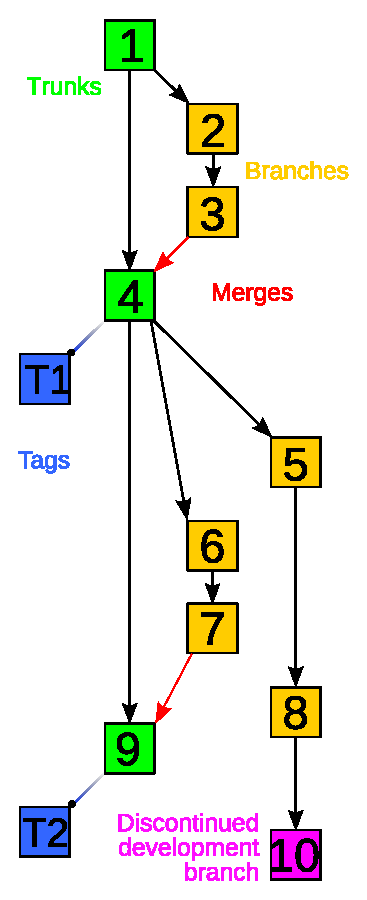
\includegraphics[height=8cm]{Revision_controlled_project_visualization-2010-24-02}\\
 \end{minipage}\\
}

\section{Issue tracker}
\frame{\frametitle{}\begin{centering}\LARGE\insertsectionhead\\\end{centering}}

\frame[containsverbatim]{ \frametitle{Issue tracker}
 \begin{itemize}
  \item Synonyms: trouble ticket system, support ticket or incident ticket system
  \item More restricted: bug tracking system, bug tracker
  \item Database of ``tickets'', describing issues/incidents/bugs
 \end{itemize}
 Workflow
 \begin{enumerate}
  \item User notices bug/issue/problem
  \item (User tries to create small test case, presenting the problem)
  \item User creates/opens ticket in issue tracker
  \item Developer reproduces problem
  \item Developer fixes problem
  \item Developer closes ticket, notifying User
 \end{enumerate}
}

\frame[containsverbatim]{ \frametitle{Issue tracker}
 Tickets/Issues can have attached
 \begin{itemize}
  \item Type (e.g. defect/enhancement)
  \item Priority (e.g. minor, major, critical, blocker)
  \item Project component
  \item Target project milestone
  \item Version of project component
  \item List of people CC'ed on changes of ticket
  \item Owner
  \item Files (e.g. patches)
 \end{itemize}
 Benefits of issue trackers over, e.g. direct developer contact
 \begin{itemize}
  \item Issues are recorded in database, cannot be forgotten
  \item Users can look-up if specific problem was already reported
  \item Users can automatically get change notifications
 \end{itemize}
}

\frame[containsverbatim]{ \frametitle{Issue tracker}
 \begin{itemize}
  \item A large number of stand-alone issue tracker implementations exist
   \begin{itemize}
    \item Trac
    \item Bugzilla
    \item GNATS
   \end{itemize}
  \item Open-source hosting sites usually automatically provide issue
        tracking systems, e.g.
   \begin{itemize}
    \item sourceforge
    \item savannah
    \item seul
    \item github
    \item google code
   \end{itemize}
 \end{itemize}
}

\section{Documentation format}
\frame{\frametitle{}\begin{centering}\LARGE\insertsectionhead\\\end{centering}}

\frame[containsverbatim]{ \frametitle{Documentation format}
 Depending on need, various formats possible
 \begin{itemize}
  \item Plain text
  \item Man pages / Help system documents
  \item Application-internal
  \item Print-oriented, e.g. \LaTeX, word processor
  \item Wiki
  \item Website as in plain HTML and typically in RCS
 \end{itemize}
}

\section*{Summary}

\frame{\frametitle{}\begin{centering}\LARGE\insertsectionhead\\\end{centering}}

\frame[containsverbatim]{ \frametitle{Summary}
 User- and development-friendly project environment provides:
 \begin{itemize}
  \item Information about project: e.g. website
  \item Communication channels for developers
  \item Infrastructure for shared code development
   \begin{itemize}
    \item Project standards
    \item Revision control system
   \end{itemize}
  \item Communication channels for users, especially
   \begin{itemize}
    \item Channel for problems/issues, directed at developers
    \item Users-for-users channel
   \end{itemize}
 \end{itemize}
}

\section{Best Coding Practices}
\frame{\frametitle{}\begin{centering}\LARGE\insertsectionhead\\\normalsize or\\\Large
 How not to annoy your collaborators\\\end{centering}}

\frame[containsverbatim]{ \frametitle{Overview}
 Best Coding Practices - Don't just do it... do it right!\\[2em]
 \begin{itemize}
  \item Project planning
   \begin{itemize}
    \item First of all: have a plan!
   \end{itemize}
  \item Programming styles and conventions
   \begin{itemize}
    \item Improve readability (to others and yourself)
    \item Reduce the probability of (you) introducing errors
    \item Make contributions by others more likely
   \end{itemize}
 \end{itemize}
}

\section{Project Planning}
\frame{\frametitle{}\begin{centering}\LARGE\insertsectionhead\\\end{centering}}

\frame[containsverbatim]{ \frametitle{Some day on Geek \& Poke}
 \begin{centering}
  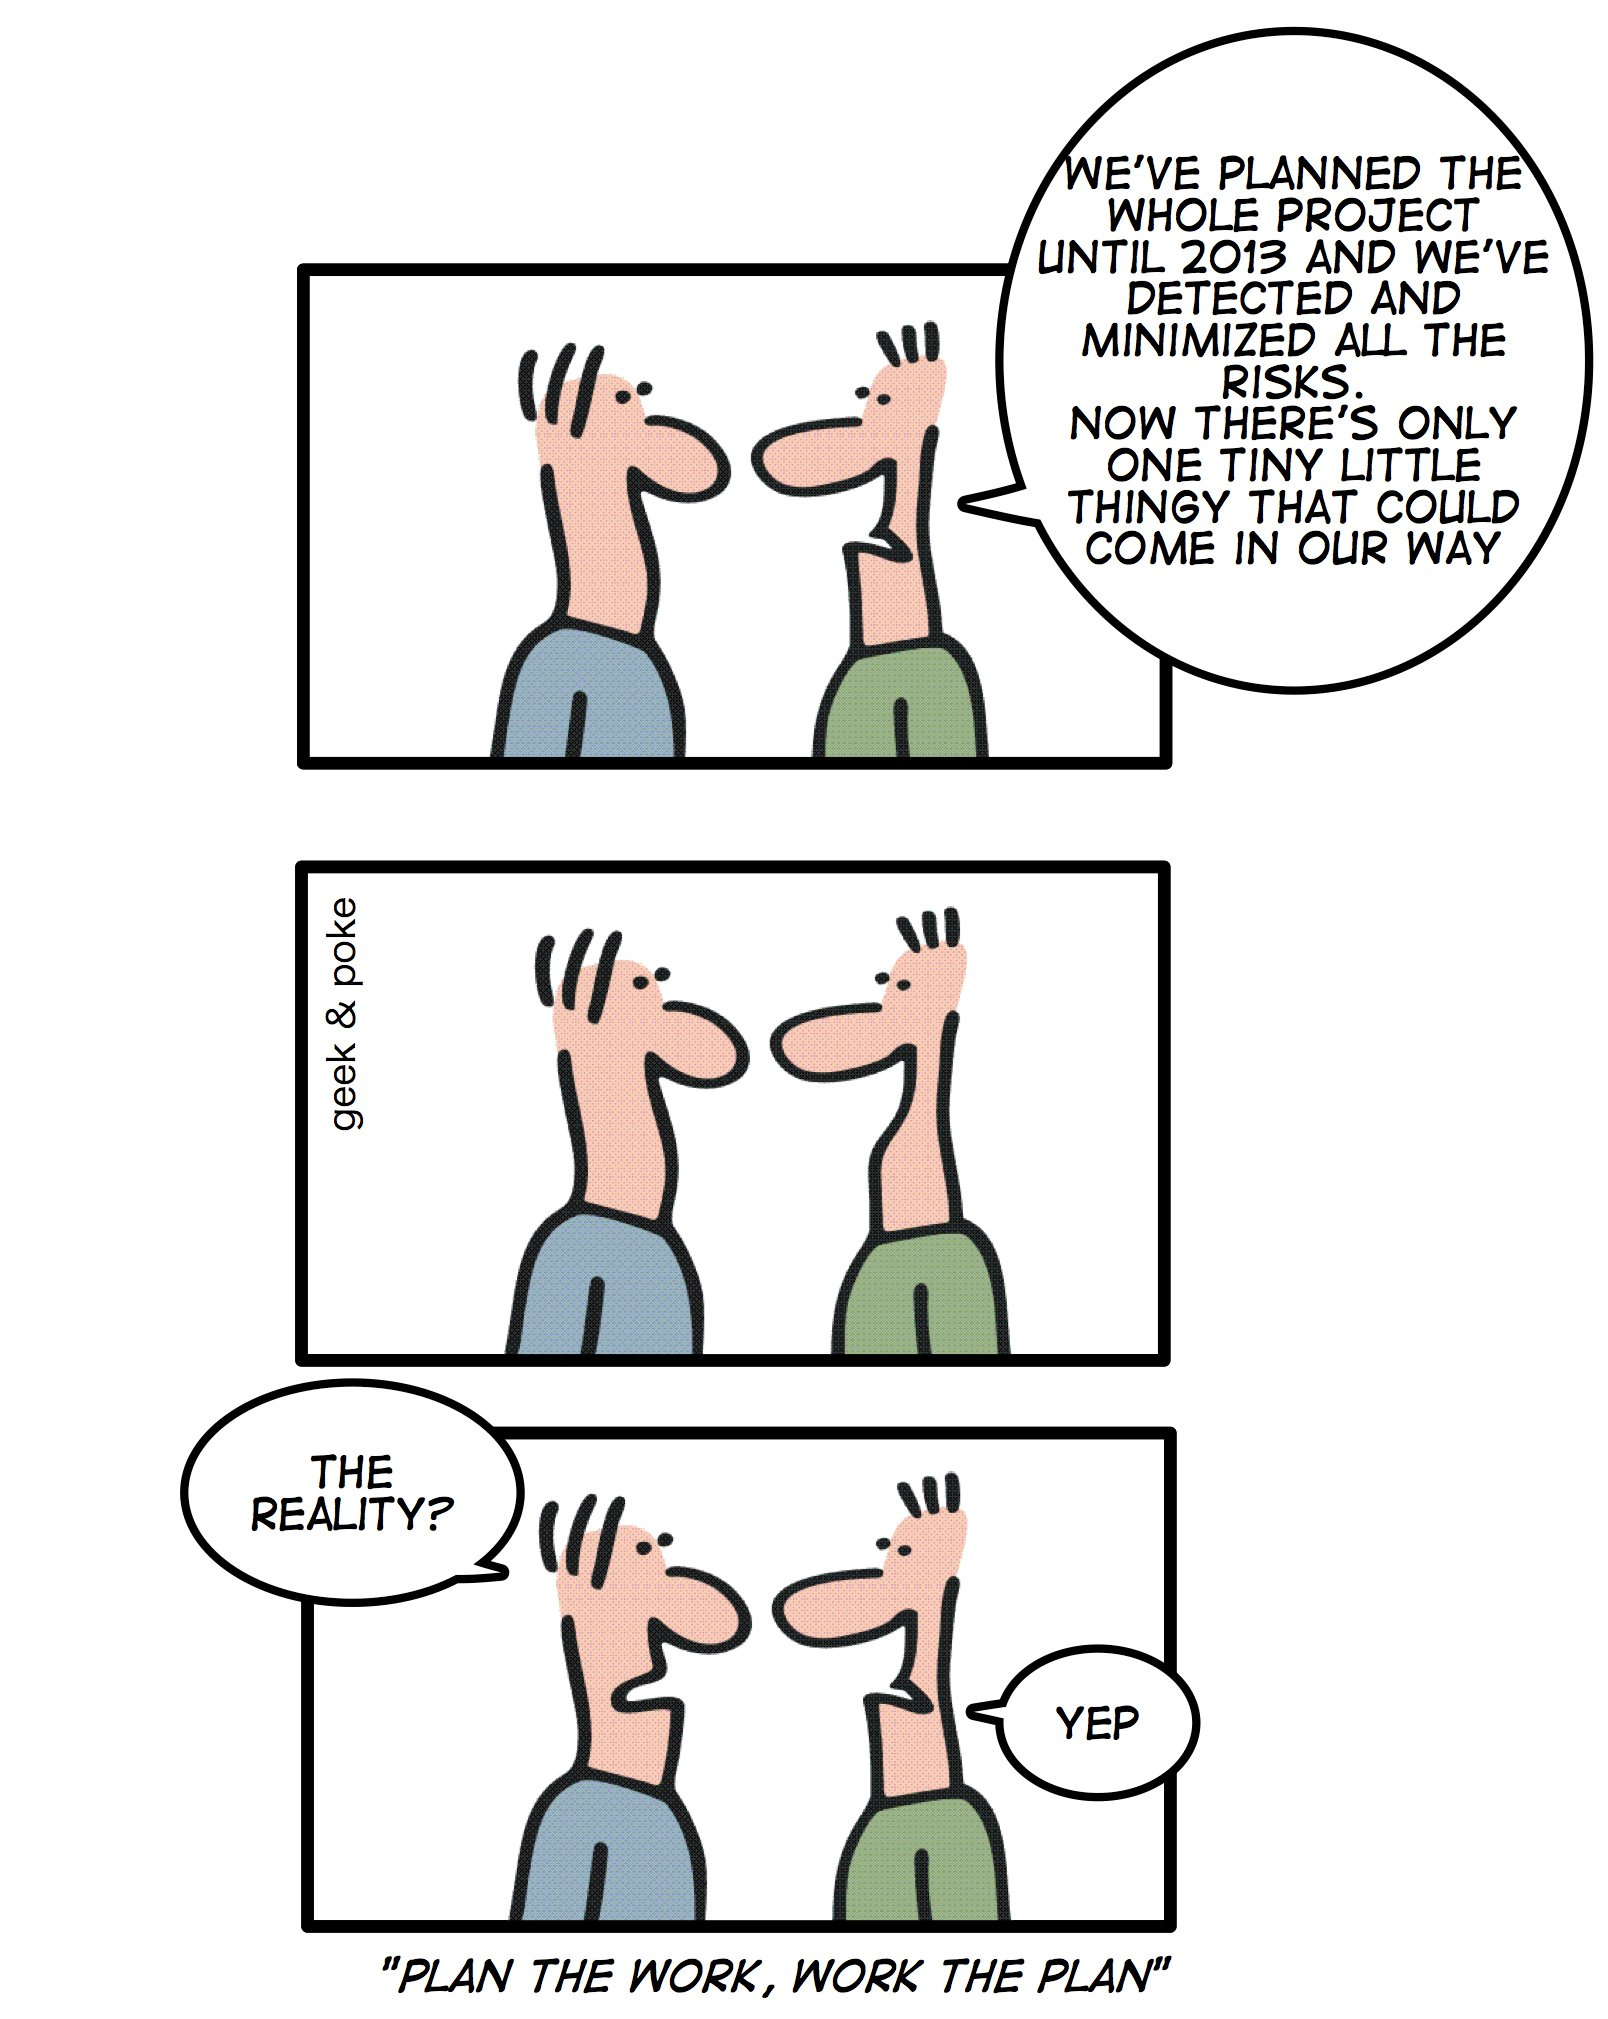
\includegraphics[height=8cm]{geek_and_poke_planning}\\
 \end{centering}
 \vspace{-0.5cm}
 \tiny http://geekandpoke.typepad.com/
}

\frame[containsverbatim]{ \frametitle{General Planning / Designing}
 Plan ahead!
 \begin{itemize}
  \item Define goals
  \item Define sub-goals
  \item Define road-map
  \item Bad plan often is better than having none
  \item The complete team must understand plan before start
  \item Do not deviate without reason
 \end{itemize}
 Design pitfalls
 \begin{itemize}
  \item Over-designing: 'Don't bite off more than you can chew'
  \item Two generally good principles
   \begin{itemize}
    \item "Keep it Simple, Stupid!" - KISS
    \item Utilize information hiding
   \end{itemize}
 \end{itemize}
}

\frame[containsverbatim]{ \frametitle{KISS}
 KISS is acronym for
 \begin{itemize}
  \item Keep it simple, Stupid!
  \item Keep it short and simple
 \end{itemize}
 Key points:
 \begin{itemize}
  \item Simplicity should be a key goal in design
  \item Unnecessary complexity should be avoided
 \end{itemize}
 Related concepts:
 \begin{itemize}
  \item Occam's razor (We should tend towards simpler theories)
  \item Einstein: \textit{``Everything should be made as simple as possible, but no simpler.''}
  \item Antoine de Saint Exupéry: \textit{``It seems that perfection is reached not when
        there is nothing left to add, but when there is\\nothing left to take away.''}
 \end{itemize}
}

\frame{ \frametitle{Code review}
 Code review / Peer review:
 \begin{itemize}
  \item Look at other peoples work. Learn from it.
  \item Solutions for problems often available - use them.
  \item Let others see your code and learn from their knowledge.
  \item Sometimes: program together (walk-through, pair programming)
 \end{itemize}
}

\section{Testing}
\frame{\frametitle{}\begin{centering}\LARGE\insertsectionhead\\\end{centering}}

\frame[containsverbatim]{ \frametitle{Testing}
 \LARGE
 \begin{itemize}
  \item Should not be an afterthought
  \item Integral part of software development
  \item Needs to be planned, and done proactively
  \item Developed while the application is being designed and coded
 \end{itemize}
}

\frame[containsverbatim]{ \frametitle{Testing}
 Functional testing
 \begin{itemize}
  \item Verify specific action or function of code
  \item Usually found in code requirements documentation
  \item ``Can the user do this''
 \end{itemize}
 Non-functional testing
 \begin{itemize}
  \item Not related to specific action or function, e.g.
  \begin{itemize}
   \item Scalability
   \item Testability
   \item Maintainability
   \item Usability
   \item Performance
   \item Security
  \end{itemize}
 \end{itemize}
}

\frame[containsverbatim]{ \frametitle{Today on Geek \& Poke}
 \begin{centering}
  
\includegraphics[height=7.5cm]{geek_and_poke_testing}\\
 \end{centering}
 \vspace{-0.5cm}
 \tiny http://geekandpoke.typepad.com/
}

\section{Source specific coding styles}

\subsection*{Identifier naming}
\frame{\frametitle{}\begin{centering}\LARGE\insertsectionhead\\\Large\insertsubsectionhead\\\end{centering}}

\frame[containsverbatim]{ \frametitle{Naming conventions}
 Reasons:
 \begin{itemize}
  \item to reduce the effort needed to read and understand source code
  \item to enhance source code appearance\\
        (for example, by disallowing overly long names or abbreviations)
  \item to enhance clarity in cases of potential ambiguity
  \item to help avoid "naming collisions" that might occur when the work product
        of different organizations is combined
 \end{itemize}
}

\frame[containsverbatim]{ \frametitle{Identifier length}
 Considerations:
 \begin{itemize}
  \item shorter identifiers may be preferred because they are easier to type
  \item extremely short identifiers are very difficult to uniquely distinguish using
        automated search and replace tools
  \item longer identifiers may be preferred because short identifiers cannot encode enough information or appear too cryptic
  \item longer identifiers may be disfavored because of visual clutter
 \end{itemize}
}

\frame[containsverbatim]{ \frametitle{Identifier length}
 Programmers generally tended to use short identifiers, in part because of
 \begin{itemize}
  \item programming languages with length limitations
  \item early linkers which required variable names to be restricted to 6 characters to save memory
  \item early source code editors lacking auto-complete
  \item early low-resolution monitors with limited line length (e.g. only 80 characters)
  \item much of computer science originating from mathematics, where variable names are often only a single letter
 \end{itemize}
}

\frame[containsverbatim]{ \frametitle{Identifier length example}
 Compare\small
 \begin{verbatim}
          get a b c 
           
          if a < 24 and b < 60 and c < 60
            return true
          else
            return false
 \end{verbatim}
 \normalsize to\small
 \begin{verbatim}
          get hours minutes seconds 
           
          if hours < 24 and minutes < 60 and seconds < 60
            return true
          else
            return false
 \end{verbatim}
}

\frame[containsverbatim]{ \frametitle{Naming Conventions}
 A set of rules for choosing identifiers
 \begin{itemize}
  \item Hungarian Notation
   \begin{itemize}
    \item embed information (e.g. type) into name
    \item lower case mnemonics
    \item examples: \verb|sName, strName, iMax, intMax, i_max|
    \item popular primarily in Microsoft environments
   \end{itemize}
  \item Underscore style
   \begin{itemize}
    \item underscore ``\verb|_|'' between compound words
    \item might be confused with minus sign
    \item underscore inconvenient on some keyboard layouts
   \end{itemize}
  \item CamelCase
   \begin{itemize}
    \item compound words, joined without spaces, capitalized words
    \item uses less characters than underscore notation
    \item inappropriate for case-insensitive languages
   \end{itemize}
 \end{itemize}
}

\subsection*{Source code formatting}
\frame{\frametitle{}\begin{centering}\LARGE\insertsectionhead\\\Large\insertsubsectionhead\\\end{centering}}

\frame[containsverbatim]{ \frametitle{Source code formatting}
 Source code formatting \textit{or} Programming style
 \begin{itemize}
  \item Often designed for a specific programming language
  \item Large projects or companies usually define style
 \end{itemize}
 Common elements
 \begin{itemize}
  \item Layout of source code, including indentation
  \item Use of white space around operators and keywords
  \item Naming Conventions
  \item Use and style of comments
  \item Use or avoidance of particular programming constructs
 \end{itemize}
}

\frame[containsverbatim]{ \frametitle{Some day on Geek \& Poke}
 \begin{centering}
  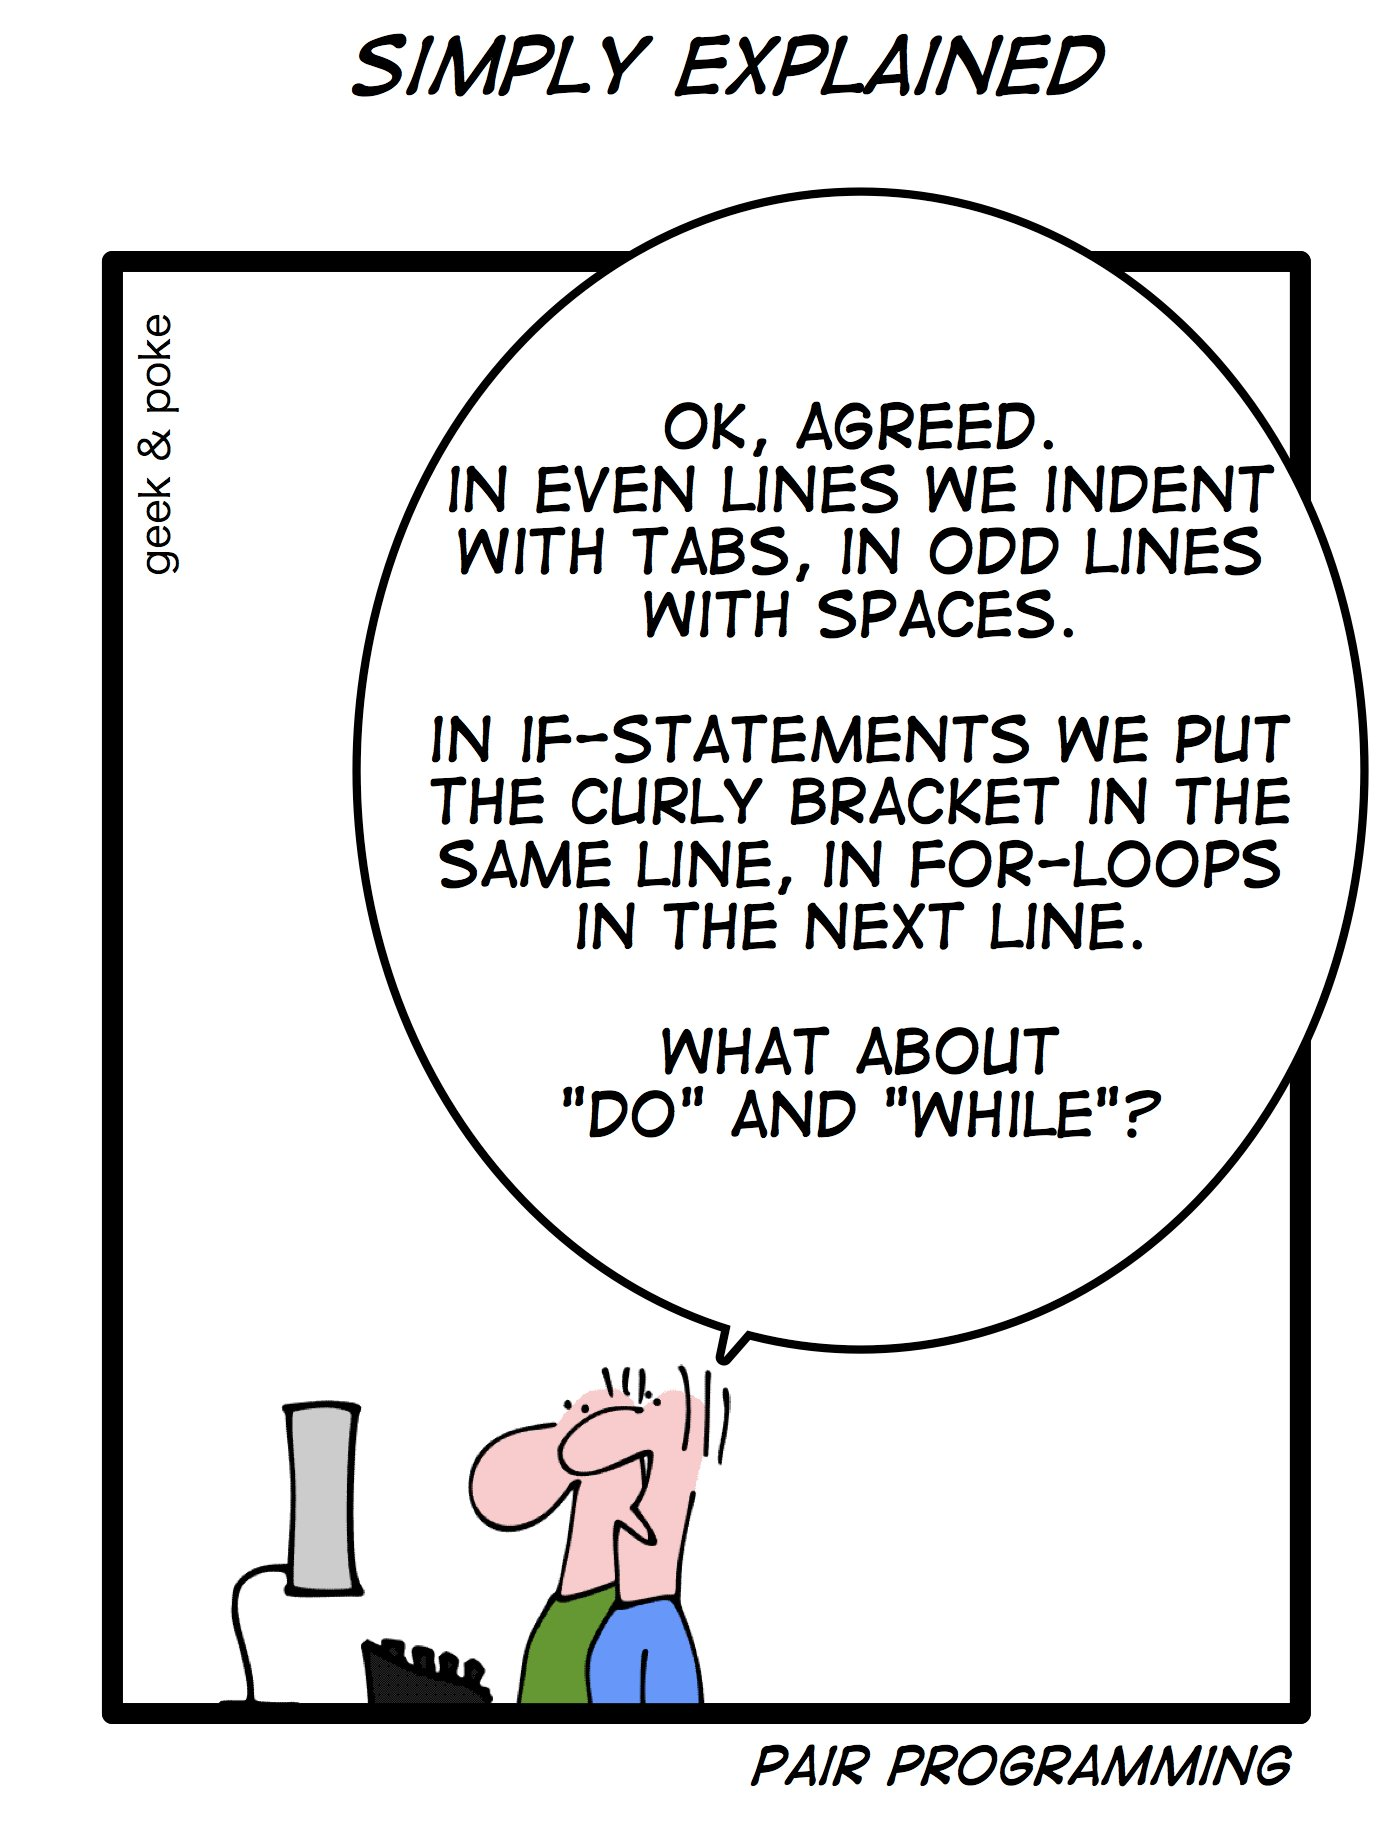
\includegraphics[height=8cm]{geek_and_poke_formatting}\\
 \end{centering}
 \vspace{-0.5cm}
 \tiny http://geekandpoke.typepad.com/
}

\frame[containsverbatim]{ \frametitle{Indent style}
 \begin{itemize}
  \item Assists in identifying control flow and blocks of code
  \item Mandatory in some programming languages
 \end{itemize}
 Compare\tiny
\begin{lstlisting}[language=C++]
          if (hours < 24 && minutes < 60 && seconds < 60)
          {
            return true;
          }
          else
          {
            return false;
          }
\end{lstlisting}
\normalsize or\tiny
\begin{lstlisting}[language=C++]
          if (hours < 24 && minutes < 60 && seconds < 60) {
            return true;
          } else {
            return false;
          }
\end{lstlisting}
\normalsize to\tiny
\begin{lstlisting}[language=C++]
          if  (    hours<
          24  && minutes<
          60  && seconds<
          60  )
          {return    true
          ;}         else
          {return   false
          ;}
\end{lstlisting}
}

\frame[containsverbatim]{ \frametitle{Vertical alignment}
 Vertical alignment is often helpful to arrange similar elements.\\*[1em]
 Compare\tiny
\begin{lstlisting}[language=Perl]
          $search = array('a', 'b', 'c', 'd', 'e');
          $replacement = array('foo', 'bar', 'baz', 'quux');
           
          # Another example:
           
          $value = 0;
          $anothervalue = 1;
          $yetanothervalue = 2;
\end{lstlisting}
\normalsize to\tiny
\begin{lstlisting}[language=Perl]
          $search      = array('a',   'b',   'c',   'd',   'e');
          $replacement = array('foo', 'bar', 'baz', 'quux');
           
          # Another example:
           
                    $value = 0;
             $anothervalue = 1;
          $yetanothervalue = 2;
\end{lstlisting}
}

\frame[containsverbatim]{ \frametitle{Whitespace}
 \begin{itemize}
  \item Most free-format languages unconcerned about amount of allowed whitespace
  \item Generally matter of taste
  \item Good practice: be consistent
 \end{itemize}
 \tiny
 \begin{minipage}{0.45\linewidth}
\begin{lstlisting}[language=C++]
          int i;
          for(i=0;i<10;++i){
              printf("%d",i*i+i);
          }
\end{lstlisting}
\begin{lstlisting}[language=C++]
          int i;
          for (i=0; i<10; ++i) {
              printf("%d", i*i+i);
          }
\end{lstlisting}
\end{minipage}
 \begin{minipage}{0.45\linewidth}
\begin{lstlisting}[language=C++]
          int i;
          for (i = 0; i < 10; ++i) {
              printf ("%d", i * i + i);
          }
\end{lstlisting}
\begin{lstlisting}[language=C++]
          int i;
          for( i = 0; i < 10; ++i ) {
              printf( "%d", i * i + i );
          }
\end{lstlisting}
\end{minipage}
}

\frame[containsverbatim]{ \frametitle{Tabs versus Spaces: An Eternal Holy War}
 People care about a few different things
 \begin{enumerate}
  \item Amount of screen columns code is indented
   \begin{itemize}
    \item a lot of different views (mainly 2, 4 or 8 spaces)
    \item might depend on context
   \end{itemize}
  \item How TAB characters in files are displayed on screen
   \begin{itemize}
    \item historic: move to the right until the current column is a multiple of 8
    \item many Microsoft Windows and Mac editors: same as above, but multiple of 4
    \item many editors configurable
    \item alternative: indent to the next tab stop (where tab stop is file-dependent)
   \end{itemize}
  \item What happens when the TAB key is pressed
   \begin{itemize}
    \item possibility 1: Insert TAB character as is
    \item possibility 2: Indent this line\\
          (cause the first non-whitespace character on this line\\to occur at specific column)
   \end{itemize}
 \end{enumerate}
}

\frame[containsverbatim]{ \frametitle{Tabs versus Spaces: An Eternal Holy War}
 People care about a few different things
 \begin{enumerate}
  \item Amount of screen columns code is indented\\
        \textcolor{green}{Core issue - matter of taste}
  \item How TAB characters in files are displayed on screen\\
        \textcolor{blue}{Technical issue, interoperability}
  \item What happens when the TAB key is pressed\\
        \textcolor{blue}{Technical issue, interoperability}
 \end{enumerate}
 Solutions:
 \begin{itemize}
  \item \textcolor{green}{Agreement within project}\\
  \item \textcolor{blue}{Avoid TAB characters in files} or, at least:\\
        \textcolor{blue}{Avoid TABS for alignment, use only for indentation}
 \end{itemize}
}

\subsection*{General programming practices}
\frame{\frametitle{}\begin{centering}\LARGE\insertsectionhead\\\Large\insertsubsectionhead\\\end{centering}}

\frame[containsverbatim]{ \frametitle{Left-hand comparisons}
 Remove possible errors by using left-hand comparisons:\\*[1em]
 Comparison:\small
 \begin{lstlisting}[language=C++]
// A right-hand comparison checking if $a equals 42.
if ( $a == 42 ) { ... }
// Recast, using the left-hand comparison style.
if ( 42 == $a ) { ... }
 \end{lstlisting}
 \normalsize Assignment:\small
 \begin{lstlisting}[language=C++]
// Inadvertent assignment which is often hard to debug
if ( $a = 42 ) { ... }
// Compile time error indicates source of problem
if ( 42 = $a ) { ... }
 \end{lstlisting}
}

\frame[containsverbatim]{ \frametitle{Looping and control structures}
 Use the ``right'' loop structure, for example:
 \begin{lstlisting}[language=C++]
          i = 0
          while i < 5
            print i * 2
            i = i + 1
          end while
          print "Ended loop"
 \end{lstlisting}
vs.
 \begin{lstlisting}
          for i = 0, i < 5, i=i+1
            print i * 2
          print "Ended loop"
 \end{lstlisting}
}

\frame[containsverbatim]{ \frametitle{Curly brackets and loops}
 Use curly brackets even when not necessary (depends on language), e.g.:\small
 \begin{lstlisting}[language=C++]
/* The incorrect indentation hides the fact that this
   line is not part of the loop body. */
          for (i = 0; i < 5; ++i);
/* --> */     printf("%d\n", i*2);
          printf("Ended loop");
 \end{lstlisting}
 \normalsize or\small
 \begin{lstlisting}[language=C++]
/* The incorrect indentation hides the fact that this
   line is not part of the loop body. */
          for (i = 0; i < 5; ++i)
              fprintf(logfile, "loop reached %d\n", i);
/* --> */     printf("%d\n", i*2);
          printf("Ended loop");
 \end{lstlisting}

}

\frame[containsverbatim]{ \frametitle{List separators}
  Add list separator after final element in list (where supported):
 \begin{lstlisting}[language=C++]
const char *array[] = {
    "item1",
    "item2",
    "item3",  /* still has the comma after it */
};
 \end{lstlisting}
 Benefit: Prevents syntax errors and subtle string-concatenation bugs after re-ordering
}

\frame[containsverbatim]{ \frametitle{Language specific convention examples}
 C, C++
 \begin{itemize}
  \item Keywords and standard library identifiers mostly lowercase
  \item Macro names only in upper case with underscores
  \item Names beginning with double underscores or underscore and capital letter are
        reserved for internals of implementation (standard library, compiler)
 \end{itemize}
 Perl
 \begin{itemize}
  \item Locally scoped variables and subroutine names are lowercase with underscores
  \item Subroutines and variables meant to be treated as private are prefixed with an underscore
  \item Declared constants are all caps
  \item Package names are camel case, except pragmas\\(e.g. \verb|use strict;|)
 \end{itemize}
}

\frame[containsverbatim]{ \frametitle{Language specific conventions}
  Python
 \begin{itemize}
  \item UpperCamelCase for class names
  \item lowercase\_separated\_by\_underscores for other names
 \end{itemize}
 Java
 \begin{itemize}
  \item Class names should be nouns in CamelCase.
  \item Methods should be verbs, in mixed case with the first letter lowercase,
        with the first letter of each internal word capitalized
  \item Except for variables, all instance, class, and class constants are in mixed
        case with a lowercase first letter. Internal words start with capital letters.
        Variable names should not start with underscore \_ or dollar sign \$ characters,
        even though both are allowed.
 \end{itemize}
}

\frame[containsverbatim]{ \frametitle{Comments / Documentation}
 \begin{itemize}
  \item Think about documentation before you start writing
  \item Update documentation regularly
  \item Comment often, explain what is done
   \begin{lstlisting}[language=C++]
  /* compute mass from integral over rho 
     as in paper xyz */
  double M = 0.0;
  for (int i=0; i<N; i++)
  {
      M += rho[i] * volume[i];
  }
   \end{lstlisting}
  \item Don't comment the obvious
   \begin{lstlisting}[language=C++]
  /* print user name */
  print "$username\n";
   \end{lstlisting}
 \end{itemize}
}

\frame[containsverbatim]{ \frametitle{Some day on Geek \& Poke}
 \begin{centering}
  
\includegraphics[height=8cm]{geek_and_poke_documentation}\\
 \end{centering}
 \vspace{-0.5cm}
 \tiny http://geekandpoke.typepad.com/
}

\frame{\frametitle{Obfuscation}
 \begin{itemize}
  \item Usually the opposite of good coding style
  \item Intellectual property protection
  \item Reduced security exposure
  \item Size reduction
  \item At best, merely makes it time-consuming, but not impossible, to reverse engineer a program
  \item Often depends on the particular characteristics of the platform and compiler, making
        ports difficult
 \end{itemize}
 $\rightarrow$ Don't do it \onslide<2->{- \textcolor{green}{Except for fun}}
}

\frame[containsverbatim]{ \frametitle{Obfuscation Example}
Print prime numbers less than 100:\small
 \begin{lstlisting}[language=C++]
void primes(int cap) {
  int i, j, composite;
  for(i = 2; i < cap; ++i) {
    composite = 0;
    for(j = 2; j * j <= i; ++j) 
      composite += !(i % j);
    if(!composite)
      printf("%d\t", i);
  }
}
 
int main(void) { 
  primes(100);
}
 \end{lstlisting}
}

\frame[containsverbatim]{ \frametitle{Obfuscation Example}
 Rewrite for as while. Use special values.\small
 \begin{lstlisting}[language=C++]
void primes(int cap) { 
  int i, j, composite, t = 0;
  while(t < cap * cap) {
    i = t / cap;
    j = t++ % cap;
    if(i <= 1);
    else if(!j)
      composite = j;
    else if(j == i && !composite)
      printf("%d\t",i);
    else if(j > 1 && j < i)
      composite += !(i % j);  
  }
}
 
int main(void) {
  primes(100);
}
 \end{lstlisting}
}

\frame[containsverbatim]{ \frametitle{Obfuscation Example}
 Change iteration into recursion:\tiny
 \begin{lstlisting}[language=C++]
void primes(int cap, int t, int composite) {
  int i,j;
  i = t / cap;
  j = t % cap;
  if(i <= 1)
    primes(cap,t+1,composite);
  else if(!j)
    primes(cap,t+1,j);
  else if(j == i && !composite)
    (printf("%d\t",i), primes(cap,t+1,composite));
  else if(j > 1 && j < i)
    primes(cap,t+1, composite + !(i % j));
  else if(t < cap * cap)
    primes(cap,t+1,composite);
}
 
int main(void) {
  primes(100,0,0);
}
 \end{lstlisting}
}

\frame[containsverbatim]{ \frametitle{Obfuscation Example}
 Obfuscate constructs and use meaningless variable names\tiny
 \begin{lstlisting}[language=C++]
void primes(int m, int t, int c) {
  int i,j;
  i = t / m;
  j = t % m;
  (i <= 1) ? primes(m,t+1,c) : (!j) ? primes(m,t+1,j) : (j == i && !c) ? 
  (printf("%d\t",i), primes(m,t+1,c)) : (j > 1 && j < i) ? 
  primes(m,t+1,c + !(i % j)) : (t < m * m) ? primes(m,t+1,c) : 0;
}
 
int main(void) {
  primes(100,0,0);
}
 \end{lstlisting}
}

\frame[containsverbatim]{ \frametitle{Obfuscation Example}
 Remove intermediate variables and literals\tiny
 \begin{lstlisting}[language=C++]
void primes(int m, int t, int c) {
  ((t / m) <= 1) ? primes(m,t+1,c) : !(t % m) ? primes(m,t+1, t % m) : 
  ((t % m)==(t / m) && !c) ? (printf("%d\t",(t / m)), primes(m,t+1,c)) : 
  ((t % m)> 1 && (t % m) < (t / m)) ? primes(m,t+1,c + !((t / m) % (t % m))) : 
  (t < m * m) ? primes(m,t+1,c) : 0;
}
 
int main(void) {
  primes(100,0,0); 
}
 \end{lstlisting}
 \normalsize Obfuscate names again\tiny
 \begin{lstlisting}[language=C++]
void _(int __, int ___, int ____) {
  ((___ / __) <= 1) ? _(__,___+1,____) : !(___ % __) ? _(__,___+1,___ % __) : 
  ((___ % __)==(___ / __) && !____) ? (printf("%d\t",(___ / __)), 
  _(__,___+1,____)) : ((___ % __) > 1 && (___ % __) < (___ / __)) ? 
  _(__,___+1,____ + !((___ / __) % (___ % __))) : (___ < __ * __) ? 
  _(__,___+1,____) : 0;
} 
 
int main(void) {
  _(100,0,0); 
}
 \end{lstlisting}
}

\frame[containsverbatim]{ \frametitle{Obfuscation Example}
 Remove literals\tiny
 \begin{lstlisting}[language=C++]
void _(int __, int ___, int ____, int _____) {
 ((___ / __) <= _____) ? _(__,___+_____,____,_____) : !(___ % __) ? _(__,___+_____,___%
  __, _____) : ((___ % __)==(___ / __) && !____) ? (printf("%d\t",(___ / __)), 
 _(__,___+_____,____,_____)) : ((___ % __) > _____ && (___ % __) < (___ / __)) ? 
 _(__,___+_____,____ + !((___ / __) % (___ % __)),_____) : (___ < __ * __) ? 
 _(__,___+_____,____,_____) : 0;
} 
 
int main(void) {
  _(100,0,0,1); 
}
 \end{lstlisting}
 \normalsize Remove redundant text\tiny
 \begin{lstlisting}[language=C++]
_(__,___,____,_____){___/__<=_____?_(__,___+_____,____,_____):!(___%__)?_(__,___+_____,
___%__,_____):___%__==___/__&&!____?(printf("%d\t",___/__),_(__,___+_____,____,_____)):
(___%__>_____&&___%__<___/__)?_(__,___+_____,____+!(___/__%(___%__)),_____):___<__*__?_
(__,___+_____,____,_____):0;}main(void){_(100, 0, 0, 1);}
 \end{lstlisting}
}

\frame[containsverbatim]{ \frametitle{Recreational obfuscation}
\def\Tiny{\fontsize{1pt}{1pt}\selectfont}
 \Tiny
 \begin{lstlisting}[language=C++]
#include                                     <math.h>
#include                                   <sys/time.h>
#include                                   <X11/Xlib.h>
#include                                  <X11/keysym.h>
                                          double L ,o ,P
                                         ,_=dt,T,Z,D=1,d,
                                         s[999],E,h= 8,I,
                                         J,K,w[999],M,m,O
                                        ,n[999],j=33e-3,i=
                                        1E3,r,t, u,v ,W,S=
                                        74.5,l=221,X=7.26,
                                        a,B,A=32.2,c, F,H;
                                        int N,q, C, y,p,U;
                                       Window z; char f[52]
                                    ; GC k; main(){ Display*e=
 XOpenDisplay( 0); z=RootWindow(e,0); for (XSetForeground(e,k=XCreateGC (e,z,0,0),BlackPixel(e,0))
; scanf("%lf%lf%lf",y +n,w+y, y+s)+1; y ++); XSelectInput(e,z= XCreateSimpleWindow(e,z,0,0,400,400,
0,0,WhitePixel(e,0) ),KeyPressMask); for(XMapWindow(e,z); ; T=sin(O)){ struct timeval G={ 0,dt*1e6}
; K= cos(j); N=1e4; M+= H*_; Z=D*K; F+=_*P; r=E*K; W=cos( O); m=K*W; H=K*T; O+=D*_*F/ K+d/K*E*_; B=
sin(j); a=B*T*D-E*W; XClearWindow(e,z); t=T*E+ D*B*W; j+=d*_*D-_*F*E; P=W*E*B-T*D; for (o+=(I=D*W+E
*T*B,E*d/K *B+v+B/K*F*D)*_; p<y; ){ T=p[s]+i; E=c-p[w]; D=n[p]-L; K=D*m-B*T-H*E; if(p [n]+w[ p]+p[s
]== 0|K <fabs(W=T*r-I*E +D*P) |fabs(D=t *D+Z *T-a *E)> K)N=1e4; else{ q=W/K *4E2+2e2; C= 2E2+4e2/ K
 *D; N-1E4&& XDrawLine(e ,z,k,N ,U,q,C); N=q; U=C; } ++p; } L+=_* (X*t +P*M+m*l); T=X*X+ l*l+M *M;
  XDrawString(e,z,k ,20,380,f,17); D=v/l*15; i+=(B *l-M*r -X*Z)*_; for(; XPending(e); u *=CS!=N){
                                   XEvent z; XNextEvent(e ,&z);
                                       ++*((N=XLookupKeysym
                                         (&z.xkey,0))-IT?
                                         N-LT? UP-N?& E:&
                                         J:& u: &h); --*(
                                         DN -N? N-DT ?N==
                                         RT?&u: & W:&h:&J
                                          ); } m=15*F/l;
                                          c+=(I=M/ l,l*H
                                          +I*M+a*X)*_; H
                                          =A*r+v*X-F*l+(
                                          E=.1+X*4.9/l,t
                                          =T*m/32-I*T/24
                                           )/S; K=F*M+(
                                           h* 1e4/l-(T+
                                           E*5*T*E)/3e2
                                           )/S-X*d-B*A;
                                           a=2.63 /l*d;
                                           X+=( d*l-T/S
                                            *(.19*E +a
                                            *.64+J/1e3
                                            )-M* v +A*
                                            Z)*_; l +=
                                            K *_; W=d;
                                            sprintf(f,
                                            "%5d  %3d"
                                            "%7d",p =l
                                           /1.7,(C=9E3+
                              O*57.3)%0550,(int)i); d+=T*(.45-14/l*
                             X-a*130-J* .14)*_/125e2+F*_*v; P=(T*(47
                             *I-m* 52+E*94 *D-t*.38+u*.21*E) /1e2+W*
                             179*v)/2312; select(p=0,0,0,0,&G); v-=(
                              W*F-T*(.63*m-I*.086+m*E*19-D*25-.11*u
                               )/107e2)*_; D=cos(o); E=sin(o); } }
 \end{lstlisting}
}

\section{Summary}
\frame[containsverbatim]{ \frametitle{Summary}
 Essential for project success:
 \begin{itemize}
  \item Planning, Evaluation
  \item Integrated testing
 \end{itemize}
 Main Coding style issues:
 \begin{itemize}
  \item Identifier naming
  \item Source code formatting
  \item Avoidance/Use of specific language constructs
 \end{itemize}
}

\section{Course Work A2}
\frame[containsverbatim]{\frametitle{Course Work}
 Remote machine access
 \begin{itemize}
  \item Login to one of the XSEDE machines (e.g. 'stampede') and one of the
        LSU HPC machines ('supermike II')
  \item Familiarize yourself with transfer between these machines and your local machine
 \end{itemize}
 Simple programming
 \begin{itemize}
  \item Write a short, simple (a bit more than ``hello world'') program (surprise us)
  \item Write it well
  \item Compile and run at on XSEDE/HPC machine
 \end{itemize}
 Write short report on what you did, and commit that and source (\verb|coursework/A2/|)\\*[1em]
 Deadline: \textbf{Fri Sep 13 2013}
}


\end{document}

